\documentclass[tikz, border=4pt]{standalone}
\usepackage{tikz}
\usepackage{tikz-timing}
\begin{document}
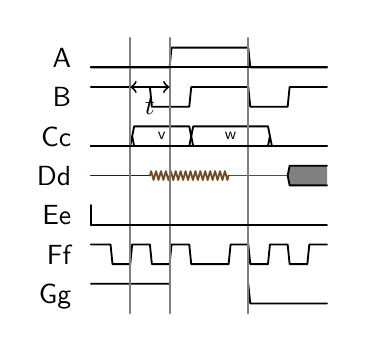
\begin{tikzpicture}[x=1cm, y=1cm]
  \node at (1.87,-1.76) {\pgfinterruptpicture%
  \begin{tikztimingtable}
    A & 4L 4H 4L \\
    B & 3H 2L 3H 2L 2H \\
    Cc & 2L 3D{v} 4D{w} 3L \\
    Dd & 3Z 4M 3X 2U \\
    Ee & 12G \\
    Ff & 3{HL} 3{LH} \\
    Gg & 4H 4S 4L \\
  \extracode
    \vertlines[gray]{2,4,8}
    \horlines{1,3,5}
    \draw [<->] (2,-1) -- node [below] {$t$} (4,-1);
  \end{tikztimingtable}%
  \endpgfinterruptpicture};
\end{tikzpicture}
\end{document}
